%
% File acl2018.tex
%
%% Based on the style files for ACL-2017, with some changes, which were, in turn,
%% Based on the style files for ACL-2015, with some improvements
%%  taken from the NAACL-2016 style
%% Based on the style files for ACL-2014, which were, in turn,
%% based on ACL-2013, ACL-2012, ACL-2011, ACL-2010, ACL-IJCNLP-2009,
%% EACL-2009, IJCNLP-2008...
%% Based on the style files for EACL 2006 by 
%%e.agirre@ehu.es or Sergi.Balari@uab.es
%% and that of ACL 08 by Joakim Nivre and Noah Smith

\documentclass[10pt,a4paper]{article}
\linespread{1}
\usepackage[hyperref]{acl2018}
\usepackage{times}
\usepackage{latexsym}
\usepackage{amsmath}

\usepackage{url}

\aclfinalcopy % Uncomment this line for the final submission
%\def\aclpaperid{***} %  Enter the acl Paper ID here

\setlength\titlebox{2.5cm}
% You can expand the titlebox if you need extra space
% to show all the authors. Please do not make the titlebox
% smaller than 5cm (the original size); we will check this
% in the camera-ready version and ask you to change it back.

\newcommand\BibTeX{B{\sc ib}\TeX}

\title{Complex Word Identification}

\author{Aneeq ur Rehman \\
  Univeristy of Sheffield  \\
  {\tt aurrehman1@sheffield.ac.uk} } 

\usepackage[export]{adjustbox}
\usepackage{amssymb}% http://ctan.org/pkg/amssymb
\usepackage{pifont}% http://ctan.org/pkg/pifont
\newcommand{\cmark}{\ding{51}}%
\newcommand{\xmark}{\ding{55}}%


\usepackage{tikz}
\def\checkmark{\tikz\fill[scale=0.4](0,.35) -- (.25,0) -- (1,.7) -- (.25,.15) -- cycle;} 

\date{}
\makeatother
\begin{document}
\maketitle




\begin{abstract}
In this paper, we present the results of a system build for complex word identification for words in Spanish and English. Depending on the features and the model used, the systems implemented predict the word complexity. We initially present a baseline system that uses some fundamental features to predict the word complexity and compare it with an improved system with additional features and models developed. Our results show that the improved system works better compared to the baseline. Finally reverse engineering is done to identify word types on which the models fail to generalize. Furthermore, suggestions are given for improving predictions on such words.
\end{abstract}

\section{Introduction}

Complex word identification is a part of lexical and text simplification. The task is to identify complex words in texts using computational methods \cite{zampieri2017complex} and to replace them with the simplest substitute to enhance the readability of text while preserving its meaning. Complex word identification targets a broad range of audience like people with aphasia, children, nonnative speaker, dyslexia  \cite{P16-1001}  or people with various cognitive and reading impairments or low literacy levels.  It has been shown that people with dyslexia read and understand better when short and frequent sentences are used. The motivation for such a system is thus targeted towards these people to simplify the text while preserving its meaning. Complex word identification is thus a binary classification problem, where a word is assigned a zero if it simple and one if it is complex.\cite{[1]} 
  \[
    c(w) = \left\{\begin{array}{lr}
        1, & \text{ \it if } w \in C\\
        0, & \text{ \it if } w \in S\\
        \end{array}\right\}
  \]
Here $w$ is the target word, $c(w)$ is a class of targeted word, $C$ is a set of complex words and $S$ is a set of simple words. We present an initial baseline system which uses four features to evaluate a word complexity and test it with different models and then develop an improved system which adds more features and combines predictions from various models. We compare our predictions with the true labels from the gold data set which is manually annoted. Our improved system shows great improvement and the finally some of the predictions where the improved system fails to predict are analyzed and suggestions are offered for future work.



\section{System Design and Implementation}
This section details about the design of the baseline and the improved system.
\subsection{Baseline}
The initial baseline system consisted of the features which were as follows:
\begin{itemize}
\item \textbf{Relative word length and word length:} 
The Relative word length was calculated by dividing the numbers of characters a word contains divided by average length of words for English and Spanish respectively. For English the average word length is 5.3 and for Spanish the average word length is 6.2. Similarly the word length was also taken as a feature. Longer words tend to be more complex and vice versa.
\item \textbf{Syllable Count:} 
The more the number of syllables a word has, the higher the complexity of that word or noun phrase. Two characters of the word were taken at time and if the first character is not in vowels and if the second one is a vowel, the syllable count was incremented by one. If the word ended with the character \texttt{e}, the total count was subtracted by one due to linguistic reasons and the count was incremented by one if the word ended with the \texttt{le}. Finally if the word did not match any of the above conditions, the count was incremented by one, i.e. a one syllable word. 
\item \textbf{Total Number of Senses:} 
The word with more senses is more ambiguous compared to a word with fewer senses. Number of senses of a word was obtained using wordnet from nltk package in python. \cite{[1]}
\end{itemize}


The system served as a baseline for the initial testing and different models were used after hyper parameter tuning through Grid Search CV and Randomized Search CV.
\subsection{Improved System}
The improved system consisted of additional features and effort was made to enrich the feature vector with high quality features. In addition to adding additional features after hyper parameter tuning, new models were added and finally a hybrid model was developed using some of the best models and this model greatly improved results. 
\subsubsection{Feature Addition}
Additional features added are as follows:
\begin{itemize}
\item \textbf{Unigram Probability:}  A huge training corpus of 0.8 billion words was taken available from the training monolingual corpus available on github containing training examples from Wikipedia, news articles, journals and the relative frequency of each of the words appearing in this corpus was calculated. This (word, probability) pair, was then stored in dictionaries which were pickled for English and Spanish respectively.  Target words from the training set were also included in these two dictionaries.
\item \textbf{Stop words and noun Phrase checks :}
The target word was also checked for being a noun phrase and stop word. Stop words were taken from nltk stop words for English and the stop words for Spanish were taken from the ranks natural language website which has different lists of texts used for various keyword analyzer tools.
\item \textbf{Vowel and Consonant Count :}
The count of vowels and consonants in a target word were also checked by iterating over the word to check for specific counts of these features, each given as lists. If a character was present in these lists, it was counted as a vowel or a consonant and the total count of these features was added up.
\item \textbf{Syonym and Hypernym count:}
In the previous case the overall senses of the word were counted by using the synsets module at word net. Now for each language and for each target word, first a check was made on whether it was a phrase and for each of the words in the noun phrase, the count of the number of synonyms and hypernyms for each word were added up and normalized by dividing by the number of words present in the phrase.
\item \textbf{BIO and POS Encoding}:
Although this feature was tested, it was excluded from testing for most part due to computational requirement needed for one hot vectors and that there was improvement using initial vectors. The POS tags and the position of each of target word in the sentence (\texttt{B},\texttt{O},\texttt{I}) was found from the spacy module and each of these tags were one hot encoded and the vectors were passed as features to the model. Spacy module also has additional features with each POS tags it uses.
\end{itemize}


\subsubsection{Model Selection and Hybrid Model Development} 
The baseline and the  improved system was initially tested on\textbf{ Decision Trees (DT)}, \textbf{Random Forest (RF)}, \textbf{K- nearest neighbours (K- nn)}, \textbf{Adaboost  Regessor} ,\textbf{ Extra Trees Regressor (ET)},\textbf{ Logistic Regression (LR)} and \textbf{Support vector machine (SVM)}  algorithms. Random Forest, decision trees, Extra Trees, Adaboost Regressors are available at scikit learn and are used because the all of these algorithms require little data preparation (i.e. normalization, blank values removal) and the cost of using the tree is logarithmic to the number of data points \cite{scikit-learn}. So this is quite useful to use. The \textbf{Hybrid Model (HM)} used here is a combination of the models that worked best combining four models (Decision Trees, Random Forest, K-neighbors, Logistic Regression). It initially relies on predictions from the K- nearest neighbors and then uses the other best models in order of performance determined earlier and predicts on the basis of these models. K-neighbors is a non-linear model used to determine if a data point will be one part of the class or the other and this model is really useful in our scenario. It looks at the neighboring points to classify the label for a data point. Performance for K- nearest neighbors also improves in general when the training data is large as its predictions are based on its neighboring points. Since the training data here for English is about 27,000 points and 13,000 points for Spanish, this model is a suitable choice to use here. For SVR, the performance did not improve significantly and the results are attached on github but testing could not be done on the test data due to run time of SVR.


\section{Testing and Experimentation}

Testing was initially done on the development data set available for both the baseline and the improved system.

\subsection{Development  Data Testing}
Table 1 below the models training results on the development data. It can be seen that firstly the performance improves significantly for the improved system with additional features. The K-nearest neighbors gives a F1 score of \textbf{0.82} for English and Random Forest gives a F1 score of \textbf{0.77} for Spanish for the improved system. This is a significant improvement in general and based on these two results, the motivation to use an ensemble hybrid model utilizing predictions from a combination of models stems. \cite{malmasi2016ltg}
\begin{table}[!htbp]
\begin{center}
\begin{tabular}{|l|rl|}
\hline \bf Model & \bf Baseline & \bf Improved  \\ \hline
DT & S:0.72, E:0.72 & S:0.76, E:0.80 \\
K-nn & S:0.70, E:0.70 & S:0.73, E:\textbf{0.82} \\
RF &  S:0.73, E:0.72  & S:\textbf{0.77}, E:0.80 \\
AB  &  S:0.71, E:0.72  & S:0.74, E:0.74 \\
ET &  S:0.73, E:0.72  & S:0.74, E:0.79 \\
LR &  S:0.69, E:0.72  & S:0.71, E:0.72 \\
\hline
\end{tabular}
\end{center}
\caption{Development Data: Baseline vs Improved System F1 Scores for English and Spanish }
\end{table}

The predictions of the baseline and the improved system on the development data were analyzed. The features outlined in Table 2 below are with the baseline mentioned in section 2.1. The table below outlines some of the target words that were present in the predictions from the baseline system which were not there in the improved system. It can be seen that the improved system, predicts better on noun phrases, common words like \texttt{President}, \texttt{profundidad} and even complex words like \texttt{exponen} and  \texttt{truce} which are as a result of incorporating unigram probabilities, noun phrase checks and additional features in the systems.

\begin{table}[!htbp]
 \begin{adjustbox}{right=7.5cm}
\begin{tabular}{|c|c|c|c|} \hline
\textbf{Word and True Label} &   \textbf{Baseline}  &  \textbf{Improved } \\ \hline
$ \texttt{\small Britain-based  \textbf{,0}}$  & \xmark &  \cmark \\ \hline
$\texttt{ \small shelling of the city \textbf{,1}}$ & \xmark  &  \cmark \\ \hline
$\texttt{ \small Vasteras \textbf{,0}}$  & \xmark  & \cmark  \\ \hline
$\texttt{\small  revered \textbf{,1}} $ & \xmark  & \cmark \\ \hline
$ \texttt{\small President \textbf{,0}} $  & \xmark & \cmark\\ \hline
$\texttt{\small  truce \textbf{,1}} $ & \xmark &  \cmark \\ \hline
$\texttt{\small encontradas \textbf{,0}}$  &  \xmark & \cmark \\ \hline
$\texttt{\small  profundidad  \textbf{,0}} $ &   \xmark &   \cmark \\ \hline
$\texttt{\small  exponen  \textbf{,1}}$  & \xmark & \cmark \\ \hline
$ \texttt{\small Mariottin \textbf{,1}} $ &\xmark &  \cmark  \\ \hline
\end{tabular}
 \end{adjustbox}
\caption{Word Predictions per System\\ \cmark= System Predicts correctly \\ \xmark= System Fails to Predict correctly}
\label{T:Features left after features with a specific percentage of Missing Values Removed}
\end{table}





\subsection{Test Data}
The Test data set was then evaluated using the baseline and the improved systems and the results were as expected. The hybrid model was also tested on the test data set and it can be seen from Table 3 below that a significant improvement in results was obtained , achieving a F1 Score of \textbf{0.91} for English and \textbf{0.87} for Spanish when models are combined together. In addition to this it can be seen that the K nearest neighbors and Random Forest work really well and serve as first point of evaluation for the hybrid model.
\begin{table}[!htbp]
\begin{center}
\begin{tabular}{|l|rl|}
\hline \bf Model & \bf Baseline & \bf Improved  \\ \hline
DT & S:0.73, E:0.71 & S:0.77, E:0.79 \\
K-nn & S:0.74, E:0.69 & S:\textbf{0.77}, E:\textbf{0.80} \\
RF &  S:0.73, E:0.71  & S:\textbf{0.77}, E:\textbf{0.80} \\
AB  &  S:0.71, E:0.71  & S:0.74, E:0.77 \\
ET &  S:0.73, E:0.71  & S:0.74, E:0.76 \\
LR &  S:0.70, E:0.71  & S:0.70, E:0.72 \\
Hybrid &  S: 0.79, E:0.78  & S:\textbf{0.87}, E:\textbf{0.91} \\
\hline
\end{tabular}
\end{center}

\caption{\label{font-table} Font guide. }
\end{table}


\subsection{Peformance Analysis}
\label{sect:pdf}

The learning curves on the test data set for different models is shown in Figure 1 and Figure 2 below for English and Spanish respectively for both the baseline and the improved system. In addition to this, the learning curve for the hybrid model was plotted for the improved system.  From Figure 1 and Figure 2, it can be seen that some models are better when the others when less training data is available for example in figure 1 for Spanish, the learning curve for baseline at n = 3000, logistic regression achieves a F1 score of \textbf{0.72} in parallel with Extra Trees and Ada boost Algorithm and K nearest neighbors achieves a F1 Score of \textbf{0.69}. It is also seen in the improved system that when n = 3000 Logistic Regression achieves a F1 Score of \textbf{0.75} and K-neighbors achieves a F1 Score of \textbf{ 0.72}. At n= 13750, when full training data, both models achieve a F1 of \textbf{0.72}. Similarly in Figure 2 for English, it can be seen that for lower amount of training data provided, the random forest algorithm \textbf{(F1:0.71)} performs better than K Neighbors \textbf{(F1:0.69)}. For Extra trees performance on the improved system improves slightly but the optimal performance is again with 9000 samples achieving a F1 of \textbf{0.75}.

\begin{figure}[!htbp]

\hspace*{0cm}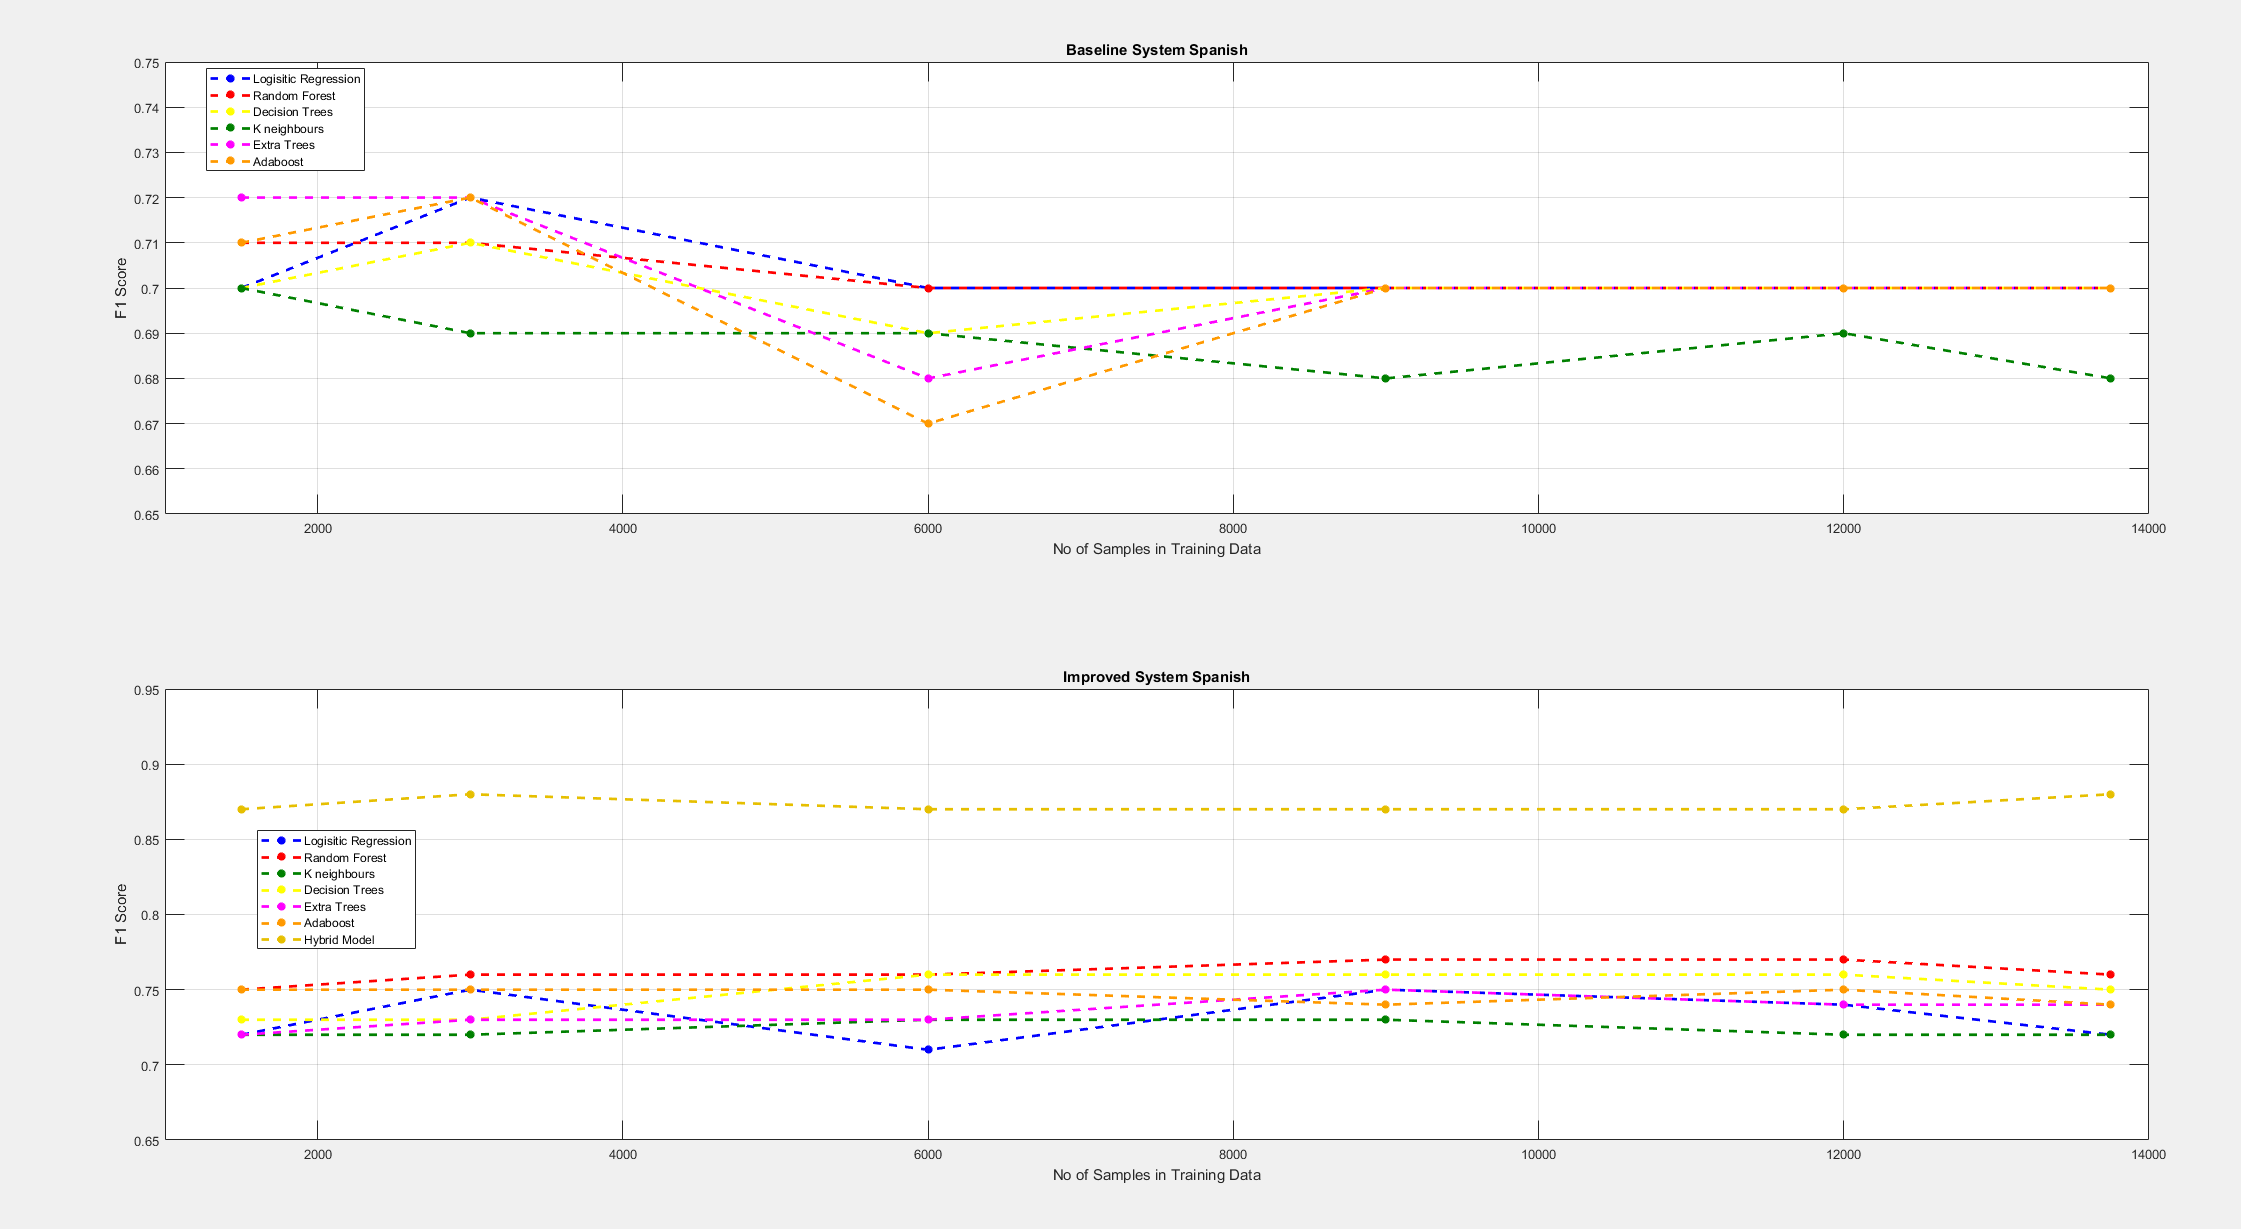
\includegraphics[width=10cm,height=8.5cm]{E:/nl/New/Capture.png}
\caption{Learning Curve Spanish: Baseline vs Imrproved }

\end{figure}
 
Similarly Figure 2 below shows the learning curve for English and it can be seen that for all the models performance generally improves except for adaboost where performance decreases slightly as more training data is available. The K-nearest algorithm achieves a F1 Score of \textbf{0.82} whereas the hybrid model achieves a F1 score of \textbf{0.91}. On the English data set, it is seen that performance improves as the number of training data samples increases.

\begin{figure}[!htbp]
\hspace*{-2cm}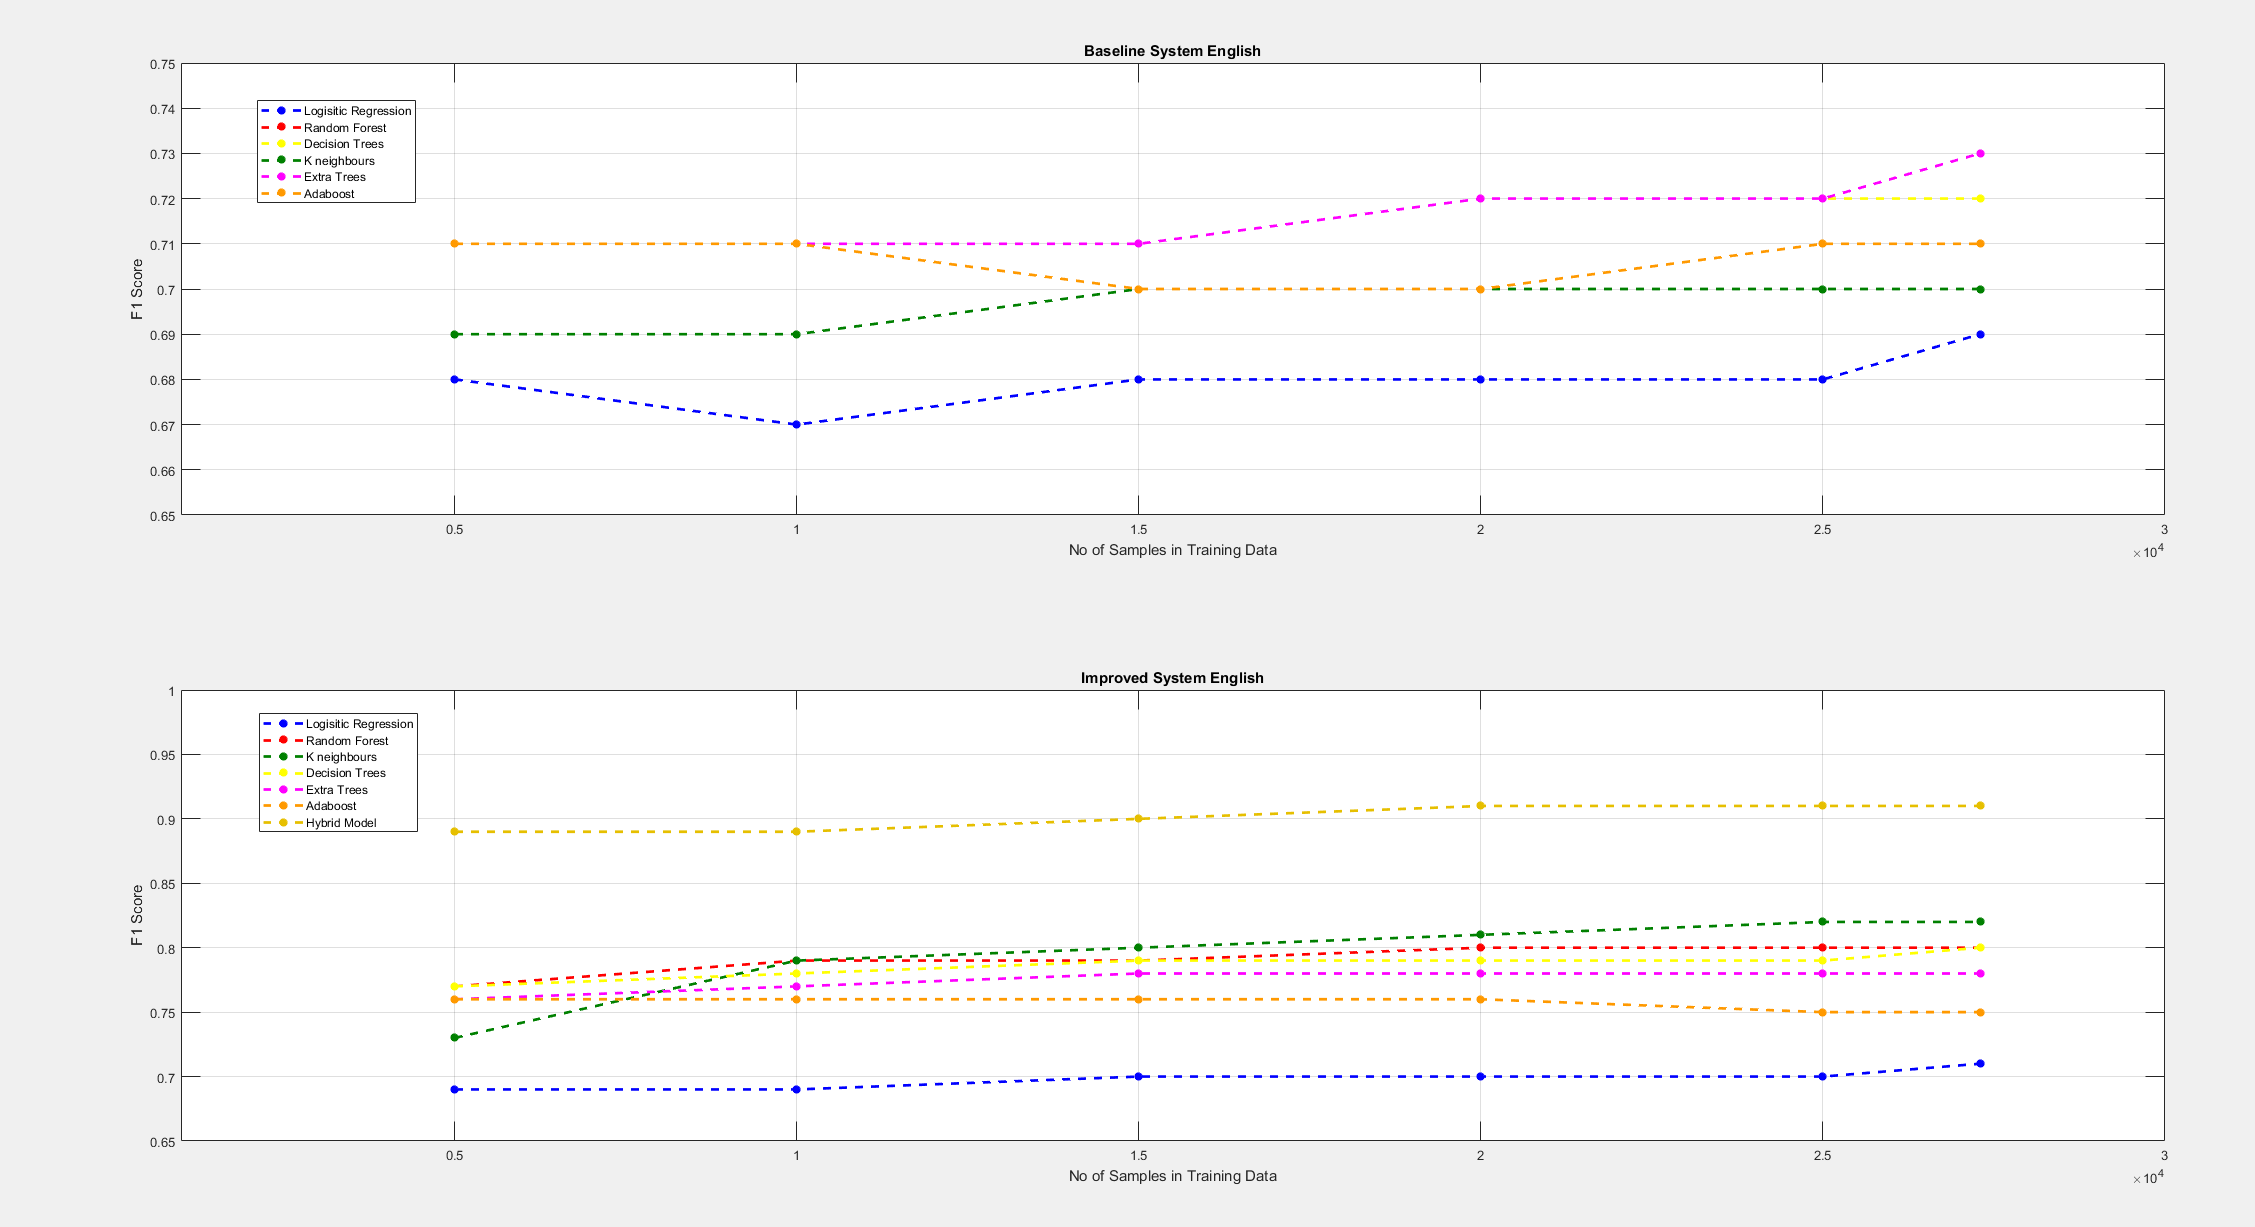
\includegraphics[width=10cm,height=8.5cm]{E:/nl/New/Capture1.png}
\caption{Learning Curve English: Baseline vs Improved }
\end{figure}


\subsection{Reverse Engineering}
\label{ssec:layout}

Finally Reverse Engineering was carried out and the predictions of the improved hybrid systems were analyzed. Table 4 below shows some of the predictions where the model failed to generalize. It can be seen that the words where the model fails to predict are very long phrases in English and some words which are very context specific, for example Sunni, Shiitte are two sects of muslims and the training on such words can be improved by having texts from various religions, cultures, ethnic origins. For Spanish some words such as regular, tribunal and musical although are the same words as in English, the training can then be provided on models for sets on words which are universal to both English and Spanish. Also words such as Guerra mean war in English, so having a training sets used for machine translation could be useful.
\begin{table}[!htbp]
\begin{adjustbox}{right=8cm}
\begin{tabular}{|c|c|c|c|} \hline
\textbf{Language Set } &   \textbf{Word} &  \textbf{Label}  \\ \hline
 English  & questioned on suspicion of assisting & 1 \\ \hline
English & Sunni  &  0 \\ \hline
English  & Afghanistan & 0  \\ \hline
English  & Shiite & 1 \\ \hline
English  &  marine surveillance ships & 0 \\ \hline
Spanish  & tribunal & 1\\ \hline
Spanish & musical & 1\\ \hline
Spanish  &  Guerra & 1 \\ \hline
Spanish  &    Longitud & 1  \\ \hline
Spanish &  regular & 0\\ \hline
Spanish &Aviacion & 1 \\ \hline
\end{tabular}
\end{adjustbox}
\caption{Examples where the Improved System Fails to generalize}
\label{T:Features left after features with a specific percentage of Missing Values Removed}
\end{table}

\subsection{Feature Selection}
Finally feature selection was done using different models, results for k-nearest neighbors are shown below in table 5.
\begin{table}[!htbp]
\begin{adjustbox}{right=10cm}
\begin{tabular}{|c|c|c|c|} \hline
\textbf{Category} &   \textbf{Features}  \\ \hline
A  & 	Syllables,Relative \& word length  , Senses \\ &  Unigram Probability\\ \hline
B & Syllables,Relative \& word length, Senses  \\ \hline
C  & Syllables,Relative \& word length  , Senses \\  &  Unigram Probability, Consonant \& Vowel Sum \\ \hline
D  & Syllables,Relative \& word length  , Senses,\\  &  Unigram Probability, Consonant \& Vowel Sum \\  & Noun Phrase, Stop words \\ \hline
E  & Syllables,Relative \& word length  , Senses, Stop words\\  &  Unigram Probability, Consonant \& Vowel Sum  \\ & ,Noun Phrase, Synonym and Hypernym count \\ \hline
\end{tabular}
\end{adjustbox}
\caption{Feature Selection}
\label{T:Features left after features}
\end{table}
As seen in figure 3 below the unigram probability has a significant impact on the model performance and set A is the best set of features with substantial improvement in model performance for both Spanish and English. Although set E offers improvement but the change is very small. Set B offers the least improvement but serves as a building block to add more features in the feature set.
\begin{figure}[!htbp]
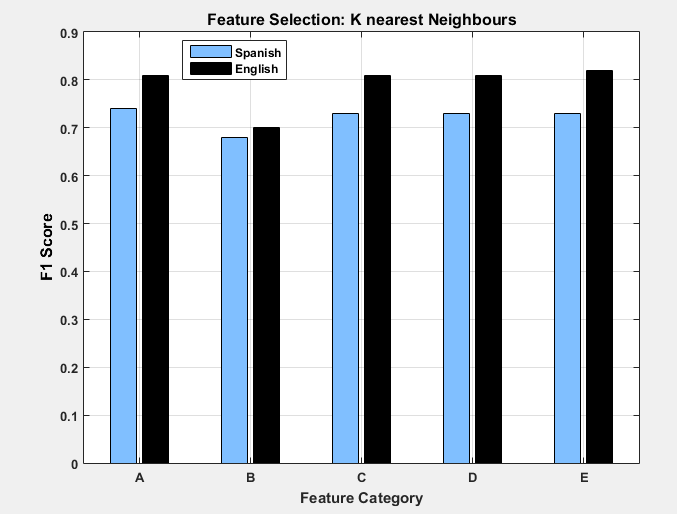
\includegraphics[width=10cm,height=6cm]{E:/nl/New/features.png}
\caption{Feature Selection: K-nn }
\end{figure}

\section{Conlusion and Future Work}
In this paper, we presented the results of a complex word identification system. We developed an initial baseline with a few rudimentary features and then we tested the system on various models and combinations of models and added additional features. Although our hybrid model results in a promising score, it still has a limitation of its dependency on the true label to make further predictions. Future work can entail developing models where ensemble methods are utilized to combine predictions from various models. Having some corpuses used in machine translation from English to Spanish or vice versa can aid model performance. Furthermore since this is a binary classification problem, implementation of neural networks could result in better models along with additional features such as bigram and trigram probabilities.








%Use 11 points for text and subsection headings, 12 points for section headings and 15 points for the title. 






%Collapse multiple citations as
%in~\cite{Gusfield:97,Aho:72}. 


















%\textbf{Placement}: Place figures and tables in the
%paper near where they are first discussed if
%possible.  
%Wide figures and tables may run across both columns and should be placed at the top of a page.



%Color illustrations are discouraged, unless you have verified that  
%they will be understandable when printed in black ink.







% include your own bib file like this:
%\bibliographystyle{acl}
%\bibliography{acl2018}
\bibliography{acl2018}
\bibliographystyle{acl_natbib}

\end{document}
